\iffalse
\let\negmedspace\undefined
\let\negthickspace\undefined
\documentclass[a4,12pt,onecolumn]{IEEEtran}
\usepackage{amsmath,amssymb,amsfonts,amsthm}
\usepackage{algorithmic}
\usepackage{graphicx}
\usepackage{textcomp}
\usepackage{xcolor}
\usepackage{txfonts}
\usepackage{listings}
\usepackage{enumitem}
\usepackage{mathtools}
\usepackage{gensymb}
\usepackage[breaklinks=true]{hyperref}
\usepackage{tkz-euclide}
\usepackage{listings}
\usepackage{circuitikz}
\usepackage{gvv}
\title{
	
	\title{NCERT Maths 11.9.2 Q9}
	\author{EE23BTECH11014- DEVARAKONDA GUNA VAISHNAVI$^{*}$% <-this % stops a space
	}
	
	
}
\begin{document}
\maketitle
	
\textbf{Question:} 
The sum of the first $n$ terms of two arithmetic progressions (AP) is in the ratio $5n+4 : 9n+6$. Find the ratio of their 18th terms.

\solution:
\fi
\begin{table}[htbp]
	\centering
    \begin{tabular}{|c|c|c|}
    \hline
    \textbf{Parameter} &\textbf{value}& \textbf{Description} \\
    \hline
    \( x_1(0) \) & $\frac{9}{2}$& First term of the first arithmetic progression (AP). \\
    \hline
    \( x_2(0) \) &$\frac{15}{2}$& First term of the second arithmetic progression (AP).  \\
    \hline
    \( d_1 \) & 5 &Common difference of the first AP. \\
    \hline
    \( d_2 \) & 9&Common difference of the second AP. \\
    \hline
    \( n \) & - &Index of the term in the sequences. \\
    \hline
    \end{tabular}
    \label{tab:parameters}
     \caption{Input Parameters}
\end{table}

\begin{align}
x_1(n)=(x_1(0)+nd_1)u(n)
\label{ncert_11.9.2.9:1}\\
x_2(n)=(x_2(0)+nd_2)u(n)
\label{ncert_11.9.2.9:2}\\
\frac{y_1(n)}{y_2(n)}=\frac{\frac{n}{2}\left[ 2x_1(0) +(n-1)d_1 \right]}{\frac{n}{2}\left[ 2x_2(0) +(n-1)d_2 \right]}&= \frac{5n+4}{9n+6}\\
\frac{2x_1(0) +nd_1-d_1}{2x_2(0) +nd_2-d_2 }&= \frac{5n+4}{9n+6}
\end{align}
\begin{center}
On comparing we get, $ d_1 = 5 $ and $ d_2 = 9$ \\
\end{center}
\begin{align}
2x_1(0) - d_1 &= 4\\
x_1(0) &=\frac{9}{2}\\
2x_2(0)- d_2&=6\\
x_2(0) &=\frac{15}{2}
\end{align}
Refer equation\eqref{eq:uz}  and equation\eqref{eq:uzder}from appendix
\begin{align}
   \implies X_1(z^{-1}) &=\frac{9/2}{1-z^{-1}} + \frac{ 5z^{-1}}{(1-z^{-1})^2}\\
    \implies X_2(z^{-1})&= \frac{15/2}{1-z^{-1}} + \frac{9z^{-1}}{(1-z^{-1})^2}\\
x_1(n)&= \lbrace 9/2,19/2,29/2,...\rbrace \\
x_2(n)&= \lbrace 15/2,33/2,51/2,...\rbrace \\
\implies \frac{x_1(18)}{x_2(18)}=\frac{179}{321}
\end{align}
\begin{figure}[h!]
	\centering
	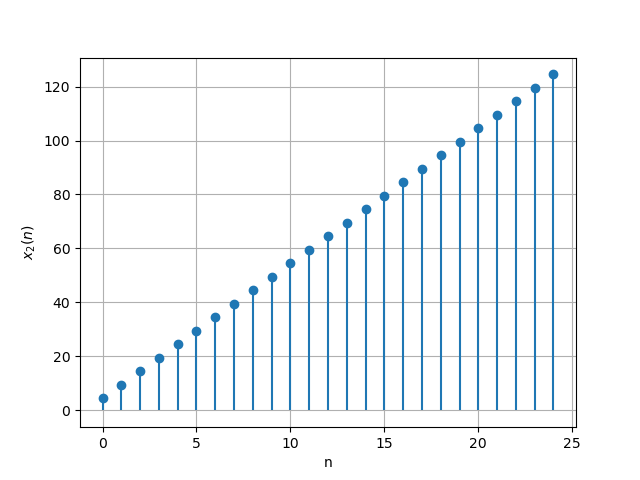
\includegraphics[width=\columnwidth]{ncert-maths/11/9/2/9/figs/fig1.png}
	\label{fig:plot}
	\caption{\large{stem plot of $x_1(n)$}}
\end{figure}
\begin{figure}[h!]
	\centering
	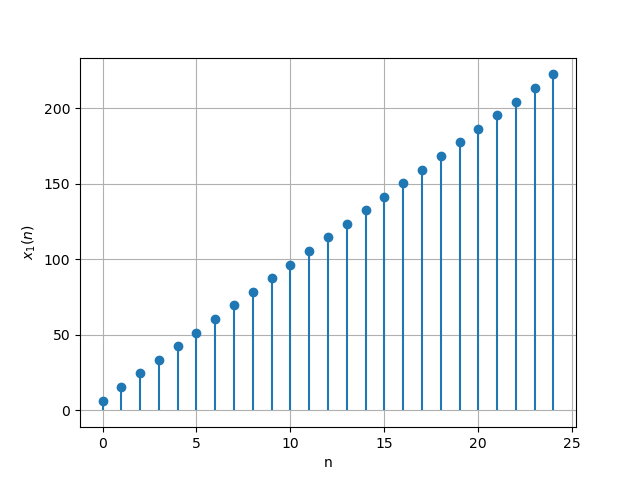
\includegraphics[width=\columnwidth]{ncert-maths/11/9/2/9/figs/fig2.png}
	\label{fig:plot}
	\caption{\large{stem plot of $x_2(n)$}}
\end{figure}
